\part{Lecture 06: Multi-Step Bootstrapping}
\title[RL Lecture 06]{Lecture 06: Multi-Step Bootstrapping}  
\date{}  
\frame{\titlepage} 

%%%%%%%%%%%%%%%%%%%%%%%%%%%%%%%%%%%%%%%%%%%%%%%%%%%%%%%%%%%%%
%% Lets Unify MC and One-Step TD Learning %%
%%%%%%%%%%%%%%%%%%%%%%%%%%%%%%%%%%%%%%%%%%%%%%%%%%%%%%%%%%%%%
\frame{\frametitle{Lets unify MC and TD learning}
\begin{figure}		
	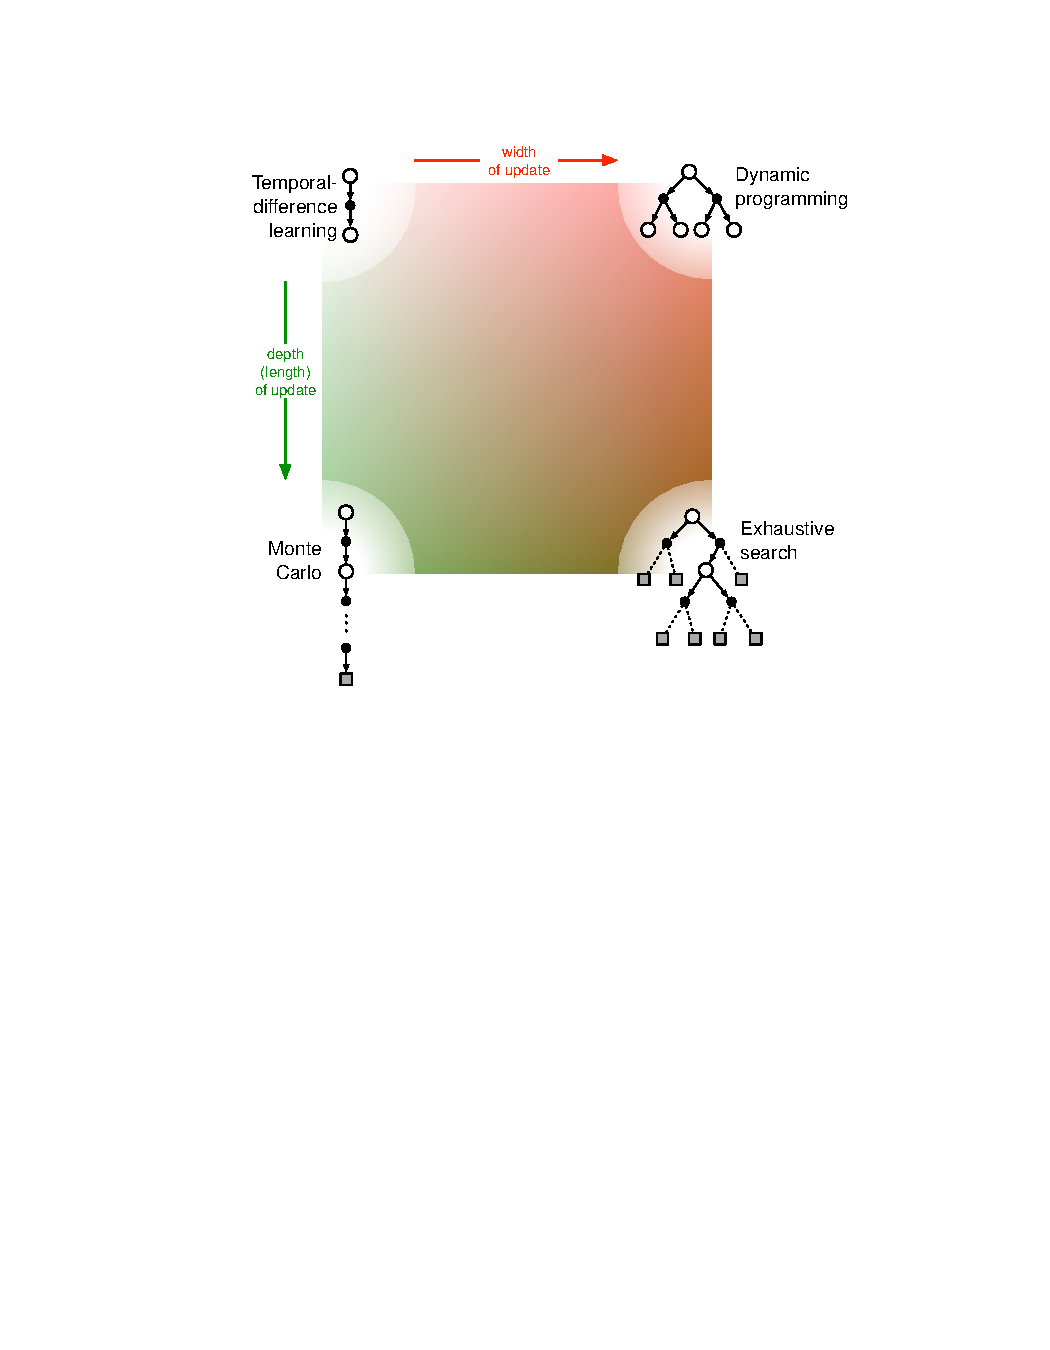
\includegraphics[height=0.65\textheight]{fig/lec06/Compare_RL_Methods_Update.pdf}
	\caption{MC and TD are the 'extreme options' in terms of the update's depth: what about intermediate solutions? (source: R. Sutton and G. Barto, Reinforcement learning: an introduction, 2018, \href{https://creativecommons.org/licenses/by-nc-nd/2.0/}{CC BY-NC-ND 2.0})}
	\label{fig:Compare_RL_Methods_Update_lec06}
\end{figure}
}

%%%%%%%%%%%%%%%%%%%%%%%%%%%%%%%%%%%%%%%%%%%%%%%%%%%%%%%%%%%%%%%%%%
\section{\texorpdfstring{$n$-step}{n-Step} TD Prediction} 
%%%%%%%%%%%%%%%%%%%%%%%%%%%%%%%%%%%%%%%%%%%%%%%%%%%%%%%%%%%%%%%%%%
\begin{frame}
\frametitle{Table of contents}
\tableofcontents
\end{frame}

%%%%%%%%%%%%%%%%%%%%%%%%%%%%%%%%%%%%%%%%%%%%%%%%%%%%%%%%%%%%%
%% n-Step Bootstrapping Idea %%
%%%%%%%%%%%%%%%%%%%%%%%%%%%%%%%%%%%%%%%%%%%%%%%%%%%%%%%%%%%%%
\frame{\frametitle{$n$-step bootstrapping idea}
\begin{columns}[t,onlytextwidth]
\begin{column}{0.6\textwidth}
\begin{minipage}[c]{\linewidth}
	\begin{figure}		
	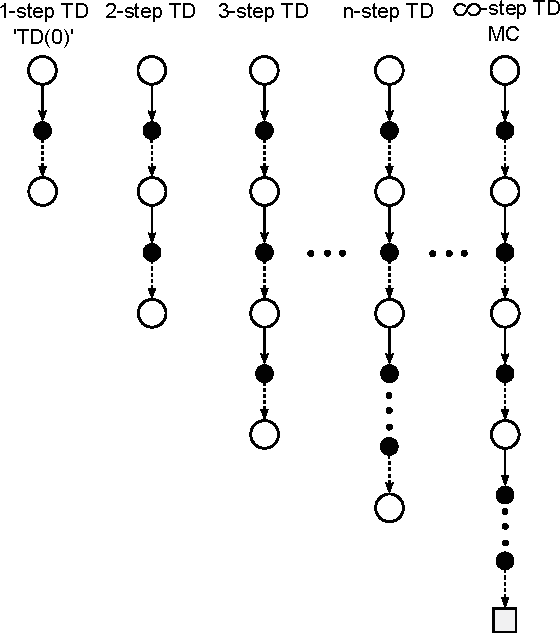
\includegraphics[height=0.65\textheight]{fig/lec06/Back_Up_n_Step_Methods.pdf}
	\caption{Different backup diagrams of $n$-step state-value prediction methods}
	\label{fig:Back_Up_n_Step_Methods}
\end{figure}
\end{minipage}
\end{column}
\hfill
\begin{column}{0.38\textwidth}
\begin{minipage}[c]{\linewidth}
	\begin{itemize}
		\item $n$-step update: consider $n$ rewards plus estimated value $n$-steps later (bootstrapping).\pause
		\item Consequence: Estimate update is available only after an $n$-step delay.\pause
		\item TD(0) and MC are special cases included in $n$-step prediction.
	\end{itemize}
\end{minipage}
\end{column}
\end{columns}
}

%%%%%%%%%%%%%%%%%%%%%%%%%%%%%%%%%%%%%%%%%%%%%%%%%%%%%%%%%%%%%
%% Formal Notation (1) %%
%%%%%%%%%%%%%%%%%%%%%%%%%%%%%%%%%%%%%%%%%%%%%%%%%%%%%%%%%%%%%
\frame{\frametitle{Formal notation (1)}
Recap the \hl{update targets} for the incremental prediction methods \eqref{eq:inc_impl_MC_pred_non_stat}:
\begin{itemize}
	\item Monte Carlo: builds on the complete sampled return series
	\begin{equation}
		g_{k:T} = r_{k+1}+\gamma r_{k+2}+\gamma^2 r_{k+3}+\cdots+\gamma^{T-k-1}r_T .
	\end{equation}
	\begin{itemize}
		\item $g_{k:T}$ denotes that all steps until termination at $T$ are considered to derive an estimate target adressing step $k$.
	\end{itemize}\pause
	\vspace{0.5cm}
	\item TD(0): utilizes a one-step bootstrapped return
	\begin{equation}
		g_{k:k+1} = r_{k+1}+\gamma \hat{v}_{k}(x_{k+1}) .
	\end{equation}
	\begin{itemize}
		\item For TD(0), $g_{k:k+1}$ highlights that only one future sampled reward step is considered before bootstrapping.
		\item $\hat{v}_{k}$ is an estimate of $v_\pi$ at time step $k$.
	\end{itemize}
\end{itemize}
}

%%%%%%%%%%%%%%%%%%%%%%%%%%%%%%%%%%%%%%%%%%%%%%%%%%%%%%%%%%%%%
%% Formal Notation (1) %%
%%%%%%%%%%%%%%%%%%%%%%%%%%%%%%%%%%%%%%%%%%%%%%%%%%%%%%%%%%%%%
\frame{\frametitle{Formal notation (2)}
\begin{block}{$n$-step state-value prediction target}
Now, the target is generalized to an arbitrary $n$-step target:
\begin{equation}
		g_{k:k+n} = r_{k+1}+\gamma r_{k+2}+\cdots+\gamma^{n-1} r_{k+n}+\gamma^{n} \hat{v}_{k+n-1}(x_{k+n}) .
\end{equation}
\end{block}\pause
\begin{itemize}
	\item Approximation of full return series truncated after $n$-steps.
	\item If $k+n \geq T$ (i.e., $n$-step prediction exceeds termination lookahead), then all missing terms are considered zero.
\end{itemize}\pause
\begin{block}{$n$-step TD}
The state-value estimate using the $n$-step return approximation is
\begin{equation}
	\hat{v}_{k+n}(x_k) = \hat{v}_{k+n-1}(x_k) + \alpha \left[g_{k:k+n} - \hat{v}_{k+n-1}(x_k)\right], \quad 0\leq k < T.
\end{equation}
\end{block}\pause
\begin{itemize}
	\item Delay of $n$-steps before $\hat{v}(x)$ is updated.
	\item Additional auxiliary update steps required at the end of each episode.
\end{itemize}
}

%%%%%%%%%%%%%%%%%%%%%%%%%%%%%%%%%%%%%%%%%%%%%%%%%%%%%%%%%%%%%
%% Convergence %%
%%%%%%%%%%%%%%%%%%%%%%%%%%%%%%%%%%%%%%%%%%%%%%%%%%%%%%%%%%%%%
\frame{\frametitle{Convergence}

\begin{theo}{Error reduction property}{error_reduction_property}
The worst error of the expected $n$-step return is always less than or equal to $\gamma^n$ times the worst error under the estimate $\hat{v}_{k+n-1}$:
\begin{equation}
	\max_x \left|\El{G_{k:k+n}|X_k = x}{\pi} - v_\pi(x)\right| \leq \gamma^n \max_x \left|\hat{v}_{k+n-1}(x) - v_\pi(x)\right| .
\end{equation}
\end{theo}\pause
\begin{itemize}
	\item Assuming an infinite number of steps/episodes and an appropriate step-size control according to \theoref{theo:converge_TD_zero}, $n$-step TD prediction converges to the true value.\pause
	\item In a more practical framework with limited number of steps/episodes:
	\begin{itemize}
		\item Choosing the best $n$-step lookahead horizon is an engineering degree of freedom.
		\item This is highly application-dependent (i.e., no predefined optimum).
		\item Prediction/estimation errors can remain due to limited data.
	\end{itemize}
\end{itemize}
}

%%%%%%%%%%%%%%%%%%%%%%%%%%%%%%%%%%%%%%%%%%%%%%%%%%%%%%%%%%%%%
%% Algorithmic Implementation: $n$-step TD-Based Prediction %%
%%%%%%%%%%%%%%%%%%%%%%%%%%%%%%%%%%%%%%%%%%%%%%%%%%%%%%%%%%%%%
\frame{\frametitle{Algorithmic implementation: $n$-step TD prediction}
\setlength{\algomargin}{0.5em}
\begin{algorithm}[H]
\small
\SetKwInput{Input}{input} 
\SetKwInput{Output}{output}
\SetKwInput{Init}{init}
\SetKwInput{Param}{parameter}
\Input{a policy $\pi$ to be evaluated, \quad \textbf{parameter:} step size $\alpha\in(0,1]$, prediction steps $n\in\mathbb{Z}^+$}
\Init{$\hat{v}(x)\, \forall \, x\in\mathcal{X}$ arbitrary except $v_0(x)=0$ if $x$ is terminal}
 \For{$j=1,\ldots,J$ episodes}{
		initialize and store $x_{0}$\;
		$T\leftarrow\infty$\;
		\Repeat( $k=0, 1, 2, \ldots$){$\tau=T-1$}{
			\If{$k<T$}{
				take action from $\pi(x_k)$, observe and store $x_{k+1}$ and $r_{k+1}$\;
				if $x_{k+1}$ is terminal: $T\leftarrow k+1$\;
				}
			$\tau\leftarrow k-n+1$ ($\tau$ time index for estimate update)\;
			\If{$\tau \geq 0$}{
				$g\leftarrow \sum_{i=\tau+1}^{\min(\tau + n, T)}\gamma^{i-\tau-1} r_i$\;
				if $\tau+n < T$: $g\leftarrow g + \gamma^n \hat{v}(x_{\tau+n})$\;
				$\hat{v}(x_{\tau}) \leftarrow \hat{v}(x_{\tau}) + \alpha\left[g - \hat{v}(x_{\tau})\right]$\;
			}
		}
	}
\caption{$n$-step TD prediction (output is an estimate $\hat{v}_\pi(x)$)}
\label{algo:TD_n_step_pred}
\end{algorithm}
}

%%%%%%%%%%%%%%%%%%%%%%%%%%%%%%%%%%%%%%%%%%%%%%%%%%%%%%%%%%%%%
%% Convergence %%
%%%%%%%%%%%%%%%%%%%%%%%%%%%%%%%%%%%%%%%%%%%%%%%%%%%%%%%%%%%%%
\frame{\frametitle{Example: 19 state random walk}
\begin{figure}		
	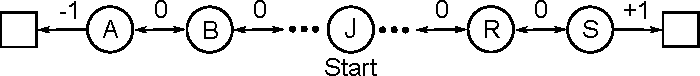
\includegraphics[height=0.1\textheight]{fig/lec06/Random_Walk_19_States.pdf}
	\caption{Exemplary random walk Markov reward process (MRP)}
	\label{fig:Random_Walk_19_States}
\end{figure}
\begin{columns}[t,onlytextwidth]
\begin{column}{0.6\textwidth}
\begin{minipage}[c]{\linewidth}
	\begin{figure}		
	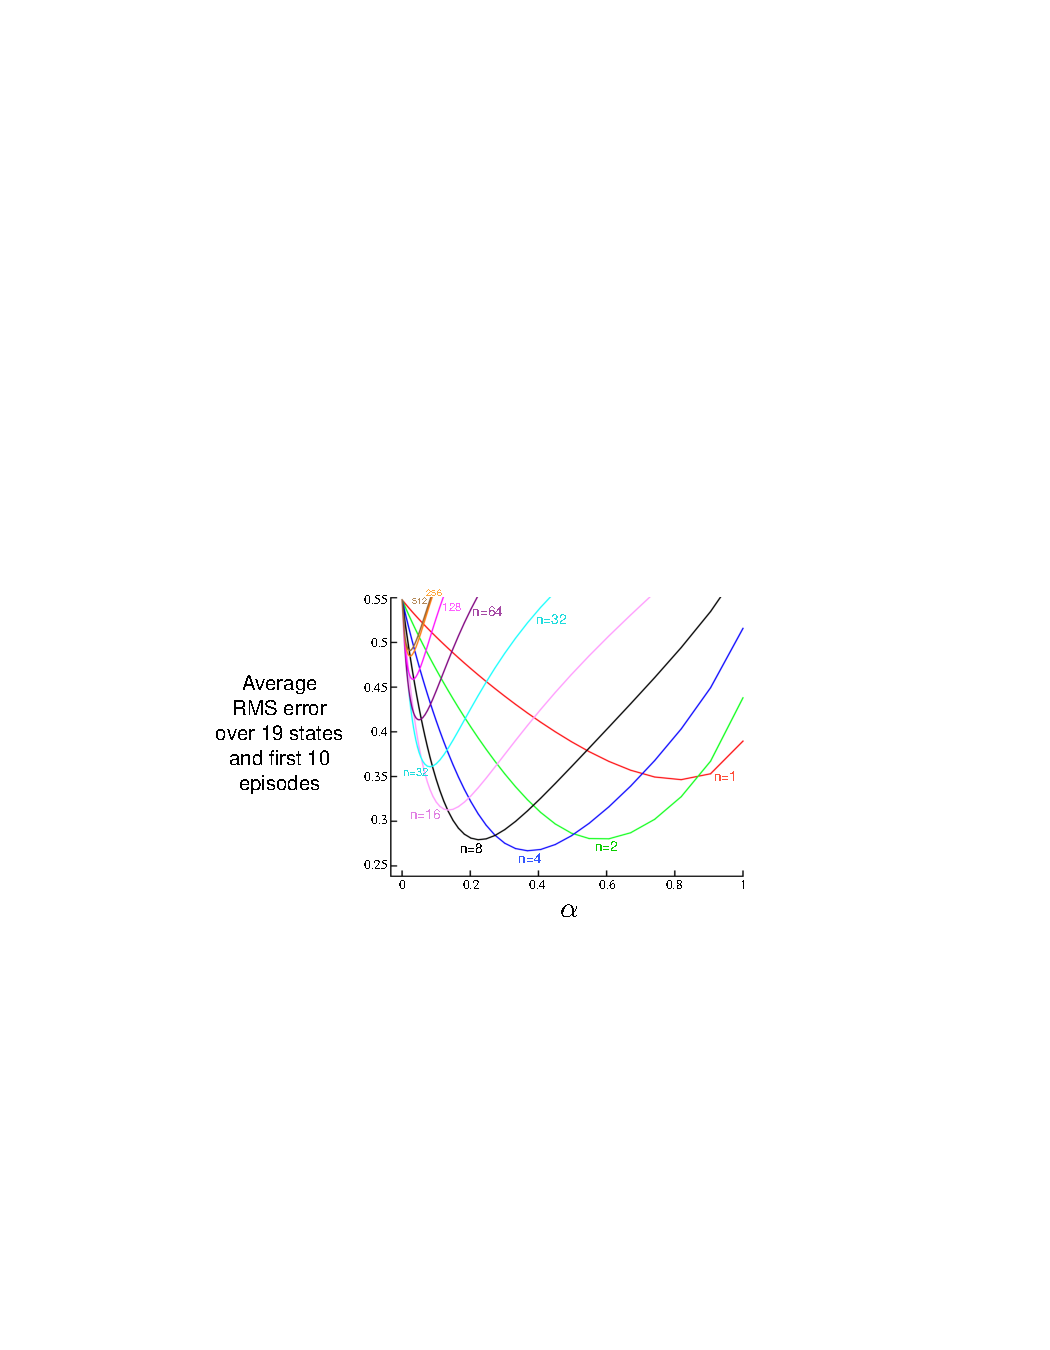
\includegraphics[height=0.45\textheight]{fig/lec06/n_Step_TD_Random_Walk.pdf}
	\caption{$n$-step TD performance (source: R. Sutton and G. Barto, Reinforcement learning: an introduction, 2018, \href{https://creativecommons.org/licenses/by-nc-nd/2.0/}{CC BY-NC-ND 2.0})}
	\label{fig:n_Step_TD_Random_Walk}
\end{figure}
\end{minipage}
\end{column}
\hfill
\begin{column}{0.38\textwidth}
\begin{minipage}[c]{\linewidth}
	\begin{itemize}
		\item Early stage performance after only 10 episodes
		\item Averaged over 100 independent runs
		\item Best result here: $n=4, \alpha \approx 0.4$
		\item Picture may change for longer episodes (no generalizable results)
	\end{itemize}
\end{minipage}
\end{column}
\end{columns}
}

%%%%%%%%%%%%%%%%%%%%%%%%%%%%%%%%%%%%%%%%%%%%%%%%%%%%%%%%%%%%%%%%%%
\section{\texorpdfstring{$n$-step}{n-Step} Control} 
%%%%%%%%%%%%%%%%%%%%%%%%%%%%%%%%%%%%%%%%%%%%%%%%%%%%%%%%%%%%%%%%%%
\begin{frame}
\frametitle{Table of contents}
\tableofcontents[currentsection]
\end{frame}

%%%%%%%%%%%%%%%%%%%%%%%%%%%%%%%%%%%%%%%%%%%%%%%%%%%%%%%%%%%%%
%% Transfer the $n$-step Approach to State-Action Values (1)%%
%%%%%%%%%%%%%%%%%%%%%%%%%%%%%%%%%%%%%%%%%%%%%%%%%%%%%%%%%%%%%
\frame{\frametitle{Transfer the $n$-step approach to state-action values (1)}
\begin{itemize}
	\item For on-policy control by SARSA action-value estimates are required. 
	\item Recap the one-step action-value update as required for 'SARSA(0)':
	\begin{equation}
		\hat{q}(x_k, u_k) \leftarrow \hat{q}(x_k, u_k) + \alpha\left[\underbrace{r_{k+1}+\gamma\hat{q}(x_{k+1}, u_{k+1})}_{\mbox{\footnotesize target }\normalsize g} - \hat{q}(x_k, u_k)\right] .
	\end{equation}
	\end{itemize}\pause
\begin{block}{$n$-step state-action value prediction target}
Analog to $n$-step TD, the state-action value target is rewritten as:
		\begin{equation}
		g_{k:k+n} = r_{k+1}+\gamma r_{k+2}+\cdots+\gamma^{n-1} r_{k+n}+\gamma^{n} \hat{q}_{k+n-1}(x_{k+n}, u_{k+n}) .
\end{equation}
\end{block}\pause
\begin{itemize}
	\item Again, if an episode terminates within the lookahead horizon ($k+n\geq T$) the target is equal to the Monte Carlo update:
	\begin{equation}
		g_{k:k+n}=g_k .
	\end{equation}
\end{itemize}
}


%%%%%%%%%%%%%%%%%%%%%%%%%%%%%%%%%%%%%%%%%%%%%%%%%%%%%%%%%%%%%
%% Transfer $n$-step Update to Action Values (2)%%
%%%%%%%%%%%%%%%%%%%%%%%%%%%%%%%%%%%%%%%%%%%%%%%%%%%%%%%%%%%%%
\frame{\frametitle{Transfer the $n$-step approach to state-action values (2)}
\begin{itemize}
	\item For $n$-step \hl{expected SARSA}, the update is similar but the state-action value estimate at step $k+n$ becomes the \hl{expected approximate value of $x$} under the target policy valid at time step $k$:
		\begin{equation}
		g_{k:k+n} = r_{k+1}+\gamma r_{k+2}+\cdots+\gamma^{n-1} r_{k+n}+\gamma^{n} \hl{\sum_u \pi(u|x)\hat{q}_k(x,u) }.
		\end{equation}\pause
\item Finally, the modified $n$-step targets can be directly integrated to the state-action value estimate update rule of Sarsa:
\end{itemize}		
\begin{block}{$n$-step SARSA}
\begin{equation}
	\hat{q}_{k+n}(x_k,u_k) = \hat{q}_{k+n-1}(x_k,u_k) + \alpha \left[g_{k:k+n} - \hat{q}_{k+n-1}(x_k, u_k)\right], \quad 0\leq k < T.
\end{equation}
\end{block}
}

%%%%%%%%%%%%%%%%%%%%%%%%%%%%%%%%%%%%%%%%%%%%%%%%%%%%%%%%%%%%%
%% $n$-Step Bootstrapping for State-Action Values %%
%%%%%%%%%%%%%%%%%%%%%%%%%%%%%%%%%%%%%%%%%%%%%%%%%%%%%%%%%%%%%
\frame{\frametitle{$n$-step bootstrapping for state-action values}
\begin{figure}		
	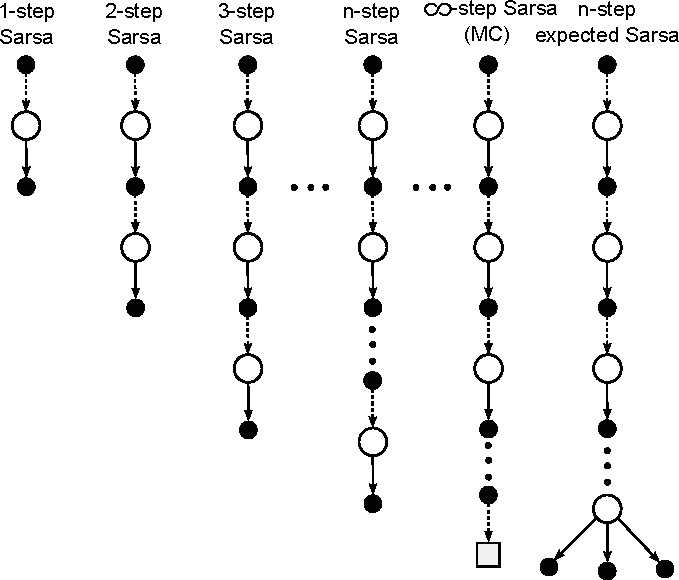
\includegraphics[height=0.75\textheight]{fig/lec06/Back_Up_n_Step_Sarsa.pdf}
	\caption{Different backup diagrams of $n$-step state-action value update targets}
	\label{fig:Back_Up_n_Step_Sarsa}
\end{figure}
}

%%%%%%%%%%%%%%%%%%%%%%%%%%%%%%%%%%%%%%%%%%%%%%%%%%%%%%%%%%%%%
%% Algorithmic Implementation: $n$-step Sarsa %%
%%%%%%%%%%%%%%%%%%%%%%%%%%%%%%%%%%%%%%%%%%%%%%%%%%%%%%%%%%%%%
\frame{\frametitle{Algorithmic implementation: $n$-step SARSA}
\setlength{\algomargin}{0.5em}
\begin{algorithm}[H]
\footnotesize
\SetKwInput{Input}{input} 
\SetKwInput{Output}{output}
\SetKwInput{Init}{init}
\SetKwInput{Param}{parameter}
%\Output{estimate $\hat{q}_\pi$ or $\hat{q}^*$}
\Param{$\alpha\in(0,1]$, $n\in\mathbb{Z}^+$, $\varepsilon\in\left\{\mathbb{R}|0<\varepsilon<<1\right\}$}
\Init{$\hat{q}(x,u)$ arbitrarily (except terminal states) $\forall \, \left\{x\in\mathcal{X}, u\in\mathcal{U}\right\}$}
\Init{$\pi$ to be $\varepsilon$-greedy with respect to $\hat{q}$ or to a given, fixed policy}
 \For{$j=1,\ldots,J$ episodes}{
		initialize $x_{0}$ and action $u_0 \sim \pi(\cdot | x_0)$ and store them\;
		$T\leftarrow\infty$\;
		\Repeat( $k=0, 1, 2, \ldots$){$\tau=T-1$}{
			\If{$k<T$}{
				take action $u_k$, observe and store $x_{k+1}$ and $r_{k+1}$\;
				\leIf{$x_{k+1}$ is terminal}{$T\leftarrow k+1$}{store $u_{k+1} \sim \pi(\cdot | x_{k+1})$}
			}
			$\tau\leftarrow k-n+1$ ($\tau$ time index for estimate update)\;
			\If{$\tau \geq 0$}{
				$g\leftarrow \sum_{i=\tau+1}^{\min(\tau + n, T)}\gamma^{i-\tau-1} r_i$\;
				if $\tau+n < T$: $g\leftarrow g + \gamma^n \hat{q}(x_{\tau+n}, u_{\tau+n})$\;
				$\hat{q}(x_{\tau},u_{\tau}) \leftarrow \hat{q}(x_{\tau},u_{\tau}) + \alpha\left[g - \hat{q}(x_{\tau}, u_{\tau})\right]$\;
				if $\pi\approx\pi^*$ is being learned, ensure $\pi(\cdot|x_\tau)$ is $\varepsilon$-greedy w.r.t to $\hat{q}$\;
			}
		}
	}
\caption{$n$-step SARSA (output is an estimate $\hat{q}_\pi$ or $\hat{q}^*$)}
\label{algo:n_step_Sarsa}
\end{algorithm}
}

%%%%%%%%%%%%%%%%%%%%%%%%%%%%%%%%%%%%%%%%%%%%%%%%%%%%%%%%%%%%%
%% Illustration with Grid-World Example %%
%%%%%%%%%%%%%%%%%%%%%%%%%%%%%%%%%%%%%%%%%%%%%%%%%%%%%%%%%%%%%
\frame{\frametitle{Illustration with grid-world example}
\begin{figure}		
	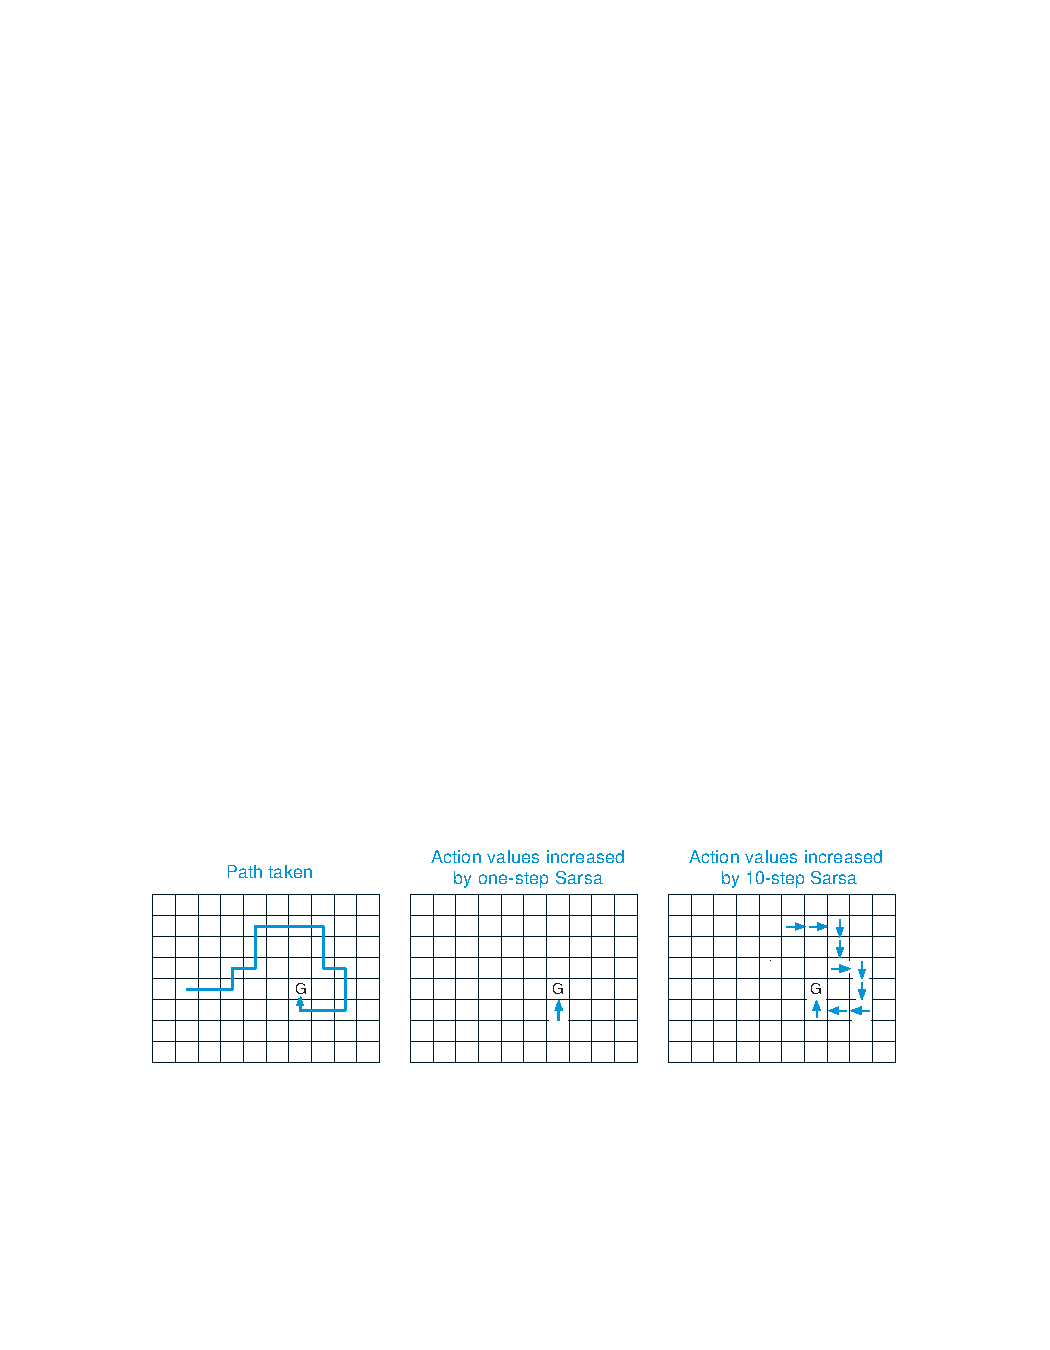
\includegraphics[height=0.35\textheight]{fig/lec06/n_step_Sarsa_Grid_World_Example.pdf}
	\caption{Executed updates (highlighted by arrows) for different $n$-step SARSA implementations during an episode (source: R. Sutton and G. Barto, Reinforcement learning: an introduction, 2018, \href{https://creativecommons.org/licenses/by-nc-nd/2.0/}{CC BY-NC-ND 2.0})}
	\label{fig:n_step_Sarsa_Grid_World_Example}
\end{figure}
\begin{itemize}
	\item For one-step SARSA, one state-action value is updated.\pause
	\item For ten-step SARSA, ten state-action values are updated.
	\item In the latter case, much more is learned during one episode.\pause
	\item Nevertheless, a trade-off between the resulting learning delay and the number of updated state-action values remains.
\end{itemize}
}

%%%%%%%%%%%%%%%%%%%%%%%%%%%%%%%%%%%%%%%%%%%%%%%%%%%%%%%%%%%%%%%%%%
\section{\texorpdfstring{$n$-step}{n-Step} Off-Policy Learning} 
%%%%%%%%%%%%%%%%%%%%%%%%%%%%%%%%%%%%%%%%%%%%%%%%%%%%%%%%%%%%%%%%%%
\begin{frame}
\frametitle{Table of contents}
\tableofcontents[currentsection]
\end{frame}

%%%%%%%%%%%%%%%%%%%%%%%%%%%%%%%%%%%%%%%%%%%%%%%%%%%%%%%%%%%%%
%% Recap on Off-Policy Learning with Importance Sampling%%
%%%%%%%%%%%%%%%%%%%%%%%%%%%%%%%%%%%%%%%%%%%%%%%%%%%%%%%%%%%%%
\frame{\frametitle{Recap on off-policy learning  with importance sampling}
Consider two separate policies in order to break the on-policy optimality trade-off:
	\begin{itemize}
		\item \hl{Behavior policy} $b(u|x)$: Explores in order to generate experience.
		\item \hl{Target policy} $\pi(u|x)$: Learns from that experience to become the optimal policy.\pause
		\item Important requirement is \hl{coverage}: Every action taken under $\pi$ must be (at least occasionally) taken under $b$, too. Hence, it follows:
	\begin{equation}
		\pi(u|x) > 0 \Rightarrow b(u|x) > 0 \quad \forall \, \left\{x\in\mathcal{X}, u\in\mathcal{U}\right\} .
	\end{equation}
	\end{itemize}\pause
\begin{block}{Importance sampling ratio (revision from \defref{defi:import_sampl_ratio})}
The relative probability of a trajectory under the target and behavior policy, the importance sampling ratio, from sample step $k$ to $T$ is:
\begin{equation}
	\rho_{k:T}=\frac{\prod_k^{T-1} \pi(u_k|x_{k})p(x_{k+1}|x_{k}, u_{k})}{\prod_k^{T-1} b(u_k|x_{k})p(x_{k+1}|x_{k}, u_{k})}=\frac{\prod_k^{T-1} \pi(u_k|x_{k})}{\prod_k^{T-1} b(u_k|x_{k})} .
\end{equation}
\end{block}
}

%%%%%%%%%%%%%%%%%%%%%%%%%%%%%%%%%%%%%%%%%%%%%%%%%%%%%%%%%%%%%
%% Transfer Importance Sampling to $n$-Step Updates %%
%%%%%%%%%%%%%%%%%%%%%%%%%%%%%%%%%%%%%%%%%%%%%%%%%%%%%%%%%%%%%
\frame{\frametitle{Transfer importance sampling to $n$-step updates}
For a straightforward \hl{$n$-step off-policy TD-style update}, just weight the update by the importance sampling ratio:
\begin{align}
	\hat{v}_{k+n}(x_k) &= \hat{v}_{k+n-1}(x_k) + \alpha \hl{\rho_{k:k+n-1}}\left[g_{k:k+n} - \hat{v}_{k+n-1}(x_k)\right], \quad 0\leq k < T, \notag \\
										\rho_{k:h}&=	\prod_k^{\min (h,T-1)}\frac{\pi(u_k|x_{k})}{b(u_k|x_{k})} .\label{eq:rho_off_policy_TD}
\end{align}
\begin{itemize}
	\item $\rho_{k:k+n-1}$ is the relative probability under the two polices taking $n$ actions from $u_k$ to $u_{k+n}$.
\end{itemize}\pause
Analog, an \hl{$n$-step off-policy SARSA-style update} exists:
\begin{equation}
\begin{split}
	\hat{q}_{k+n}(x_k,u_k) &= \hat{q}_{k+n-1}(x_k,u_k) \\&+ \alpha \hl{\rho_{k+1:k+n}}\left[g_{k:k+n} - \hat{q}_{k+n-1}(x_k, u_k)\right], \quad 0\leq k < T.
	\end{split}
\end{equation}
\begin{itemize}
	\item Here, $\rho$ starts and ends one step later compared to the TD case since state-action pairs are updated.
\end{itemize}
}

%%%%%%%%%%%%%%%%%%%%%%%%%%%%%%%%%%%%%%%%%%%%%%%%%%%%%%%%%%%%%
%% Algorithmic Implementation: Off-Policy $n$-step TD Prediction %%
%%%%%%%%%%%%%%%%%%%%%%%%%%%%%%%%%%%%%%%%%%%%%%%%%%%%%%%%%%%%%
\frame{\frametitle{Implementation: off-policy $n$-step TD-based prediction}
\vspace{-0.2cm}
\setlength{\algomargin}{0.5em}
\begin{algorithm}[H]
\small
\SetKwInput{Input}{input} 
\SetKwInput{Output}{output}
\SetKwInput{Init}{init}
\SetKwInput{Param}{parameter}
\Input{a target policy $\pi$ and a behavior policy $b$ with coverage of $\pi$}
\Param{step size $\alpha\in(0,1]$, prediction steps $n\in\mathbb{Z}^+$}
\Init{$\hat{v}(x)\, \forall \, x\in\mathcal{X}$ arbitrary except $v_0(x)=0$ if $x$ is terminal}
 \For{$j=1,\ldots,J$ episodes}{
		initialize and store $x_{0}$ and set $T\leftarrow\infty$\;
		\Repeat( $k=0, 1, 2, \ldots$){$\tau=T-1$}{
			\If{$k<T$}{
				take action from $b(x_k)$, observe and store $x_{k+1}$ and $r_{k+1}$\;
				if $x_{k+1}$ is terminal: $T\leftarrow k+1$\;
				}
			$\tau\leftarrow k-n+1$ ($\tau$ time index for estimate update)\;
			\If{$\tau \geq 0$}{
				\hl{$\rho \leftarrow \prod_{i=\tau }^{\min (\tau + n - 2,T-1)}\frac{\pi(u_i|x_{k})}{b(u_i|x_{i})}$}\;
				$g\leftarrow \sum_{i=\tau+1}^{\min(\tau + n, T)}\gamma^{i-\tau-1} r_i$\;
				if $\tau+n < T$: $g\leftarrow g + \gamma^n \hat{v}(x_{\tau+n})$\;
				$\hat{v}(x_{\tau}) \leftarrow \hat{v}(x_{\tau}) + \alpha \hl{\rho}\left[g - \hat{v}(x_{\tau})\right]$\;
			}
		}
	}
\caption{Off-policy $n$-step TD prediction (output is  an estimate $\hat{v}_\pi(x)$)}
\label{algo:TD_n_step_pred_off_policy}
\end{algorithm}
}

%%%%%%%%%%%%%%%%%%%%%%%%%%%%%%%%%%%%%%%%%%%%%%%%%%%%%%%%%%%%%
%% Algorithmic Implementation: Off-Policy $n$-step Sarsa %%
%%%%%%%%%%%%%%%%%%%%%%%%%%%%%%%%%%%%%%%%%%%%%%%%%%%%%%%%%%%%%
\frame{\frametitle{Algorithmic implementation: off-policy $n$-step SARSA}
\setlength{\algomargin}{0.5em}
\vspace{-0.15cm}
\begin{algorithm}[H]
\footnotesize
\SetKwInput{Input}{input} 
\SetKwInput{Output}{output}
\SetKwInput{Init}{init}
\SetKwInput{Param}{parameter}
\Input{an arbitrary behavior policy $b$ with $b(u|x)>0 \, \forall \, \left\{x\in\mathcal{X}, u\in\mathcal{U}\right\}$}
\Param{$\alpha\in(0,1]$, $n\in\mathbb{Z}^+$, $\varepsilon\in\left\{\mathbb{R}|0<\varepsilon<<1\right\}$}
\Init{$\hat{q}(x,u)$ $\forall \, \left\{x\in\mathcal{X}, u\in\mathcal{U}\right\}$ and a policy $\pi$ to be greedy with respect to $\hat{q}$ or to a given, fixed policy}
 \For{$j=1,\ldots,J$ episodes}{
		initialize $x_{0}$ and action $u_0 \sim b(\cdot | x_0)$ and store them, set also $T\leftarrow\infty$\;
		\Repeat( $k=0, 1, 2, \ldots$){$\tau=T-1$}{
			\If{$k<T$}{
				take action $u_k\sim b(\cdot | x_k)$, observe and store $x_{k+1}$ and $r_{k+1}$\;
				\leIf{$x_{k+1}$ is terminal}{$T\leftarrow k+1$}{store $u_{k+1} \sim b(\cdot | x_{k+1})$}
			}
			$\tau\leftarrow k-n+1$ ($\tau$ time index for estimate update)\;
			\If{$\tau \geq 0$}{
				\hl{$\rho \leftarrow \prod_{i=\tau +1}^{\min (\tau + n -1,T-1)}\frac{\pi(u_i|x_{i})}{b(u_i|x_{i})}$}\;
				$g\leftarrow \sum_{i=\tau+1}^{\min(\tau + n, T)}\gamma^{i-\tau-1} r_i$\;
				if $\tau+n < T$: $g\leftarrow g + \gamma^n \hat{q}(x_{\tau+n}, u_{\tau+n})$\;
				$\hat{q}(x_{\tau},u_{\tau}) \leftarrow \hat{q}(x_{\tau},u_{\tau}) + \alpha \hl{\rho} \left[g - \hat{q}(x_{\tau}, u_{\tau})\right]$\;
				if $\pi\approx\pi^*$ is being learned, ensure $\pi(\cdot|x_\tau)$ is $\varepsilon$-greedy w.r.t to $\hat{q}$\;
			}
		}
	}
\caption{Off-policy $n$-step SARSA (output is an estimate $\hat{q}_\pi$ or $\hat{q}^*$)}
\label{algo:n_step_Sarsa_off_policy}
\end{algorithm}
}

%%%%%%%%%%%%%%%%%%%%%%%%%%%%%%%%%%%%%%%%%%%%%%%%%%%%%%%%%%%%%%%%%%
\section{TD(\texorpdfstring{$\lambda$}{Lambda})} 
%%%%%%%%%%%%%%%%%%%%%%%%%%%%%%%%%%%%%%%%%%%%%%%%%%%%%%%%%%%%%%%%%%
\begin{frame}
\frametitle{Table of contents}
\tableofcontents[currentsection]
\end{frame}

%%%%%%%%%%%%%%%%%%%%%%%%%%%%%%%%%%%%%%%%%%%%%%%%%%%%%%%%%%%%%
%%  Averaging of $n$-Step Returns %%
%%%%%%%%%%%%%%%%%%%%%%%%%%%%%%%%%%%%%%%%%%%%%%%%%%%%%%%%%%%%%
\frame{\frametitle{Averaging of $n$-step returns}
\begin{columns}[t,onlytextwidth]
\begin{column}{0.35\textwidth}
\begin{minipage}[c]{\linewidth}
\begin{figure}
	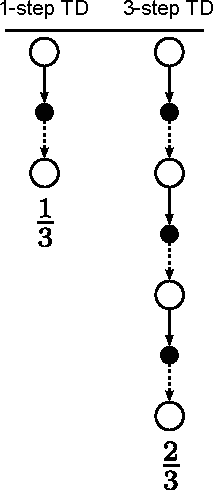
\includegraphics[height=0.65\textheight]{fig/lec06/Average_Bootstrap_Example.pdf}
	\caption{Exemplary averaging of $n$-step returns}
	\label{fig:Average_Bootstrap_Example}
\end{figure}
\end{minipage}
\end{column}
\hfill
\begin{column}{0.65\textwidth}
\begin{minipage}[c]{\linewidth}
\begin{itemize}
	\item Averaging different $n$-step returns is possible without introducing a bias (if sum of weights is one).
	\item Example on the left:
	\begin{equation*}
		g = \frac{1}{3}g_{k:k+1} + \frac{2}{3}g_{k:k+3}
	\end{equation*}
	\item Horizontal line in backup diagram indicates the averaging.\pause 
	\item Enables additional degree of freedom to reduce prediction error. \pause
	\item Such updates are called \hl{compound updates}.
\end{itemize}
\end{minipage}
\end{column}
\end{columns}
}

%%%%%%%%%%%%%%%%%%%%%%%%%%%%%%%%%%%%%%%%%%%%%%%%%%%%%%%%%%%%%
%% $\lambda$-Return (1) %%
%%%%%%%%%%%%%%%%%%%%%%%%%%%%%%%%%%%%%%%%%%%%%%%%%%%%%%%%%%%%%
\frame{\frametitle{$\lambda$-return (1)}
\begin{columns}[t,onlytextwidth]
\begin{column}{0.45\textwidth}
\begin{minipage}[c]{\linewidth}
\begin{figure}
	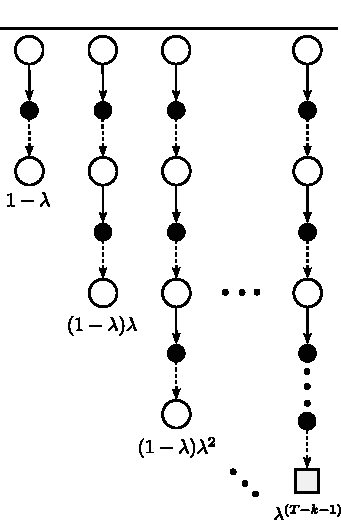
\includegraphics[height=0.7\textheight]{fig/lec06/Lambda_Return_Backup.pdf}
	\caption{Backup diagram for $\lambda$-returns}
	\label{fig:Lambda_Return_Backup}
\end{figure}
\end{minipage}
\end{column}
\hfill
\begin{column}{0.55\textwidth}
\begin{minipage}[c]{\linewidth}
\begin{itemize}
	\item \hl{$\lambda$-return}: is a compound update with exponentially decaying weights:
	\begin{equation}
		g_k^\lambda = (1-\lambda)\sum_{n=1}^{\infty}\lambda^{(n-1)}g_{k:k+n}\,.
		\label{eq:lambda_return}
	\end{equation}
	\item Parameter is $\lambda\in\left\{\mathbb{R}|0\leq \lambda \leq 1\right\}$.
	\item Geometric series of weights is one:
	\begin{equation*}
		(1-\lambda)\sum_{n=1}^{\infty}\lambda^{(n-1)} = 1
	\end{equation*}
\end{itemize}
\end{minipage}
\end{column}
\end{columns}
}

%%%%%%%%%%%%%%%%%%%%%%%%%%%%%%%%%%%%%%%%%%%%%%%%%%%%%%%%%%%%%
%% $\lambda$-Return (2) %%
%%%%%%%%%%%%%%%%%%%%%%%%%%%%%%%%%%%%%%%%%%%%%%%%%%%%%%%%%%%%%
\frame{\frametitle{$\lambda$-return (2)}
\onslide<1->{\begin{itemize}
	\item Rewrite $\lambda$-return for episodic tasks with termination at $k=T$:
		\begin{equation}
		g_k^\lambda = (1-\lambda)\sum_{n=1}^{T-k-1}\lambda^{(n-1)}g_{k:k+n} + \lambda^{T-k-1}g_k\,.
		\label{eq:lambda_return_episodic}
	\end{equation}
	\item Return $g_k$ after termination is weighted with residual weight $\lambda^{T-k-1}$.}
	\onslide<2->{\item Above, \eqref{eq:lambda_return_episodic} includes two special cases:
	\begin{itemize}
		\item If $\lambda=0$: becomes TD(0) update.
		\item If $\lambda=1$: becomes MC update.
	\end{itemize}}
\end{itemize}
\onslide<1->{\begin{figure}
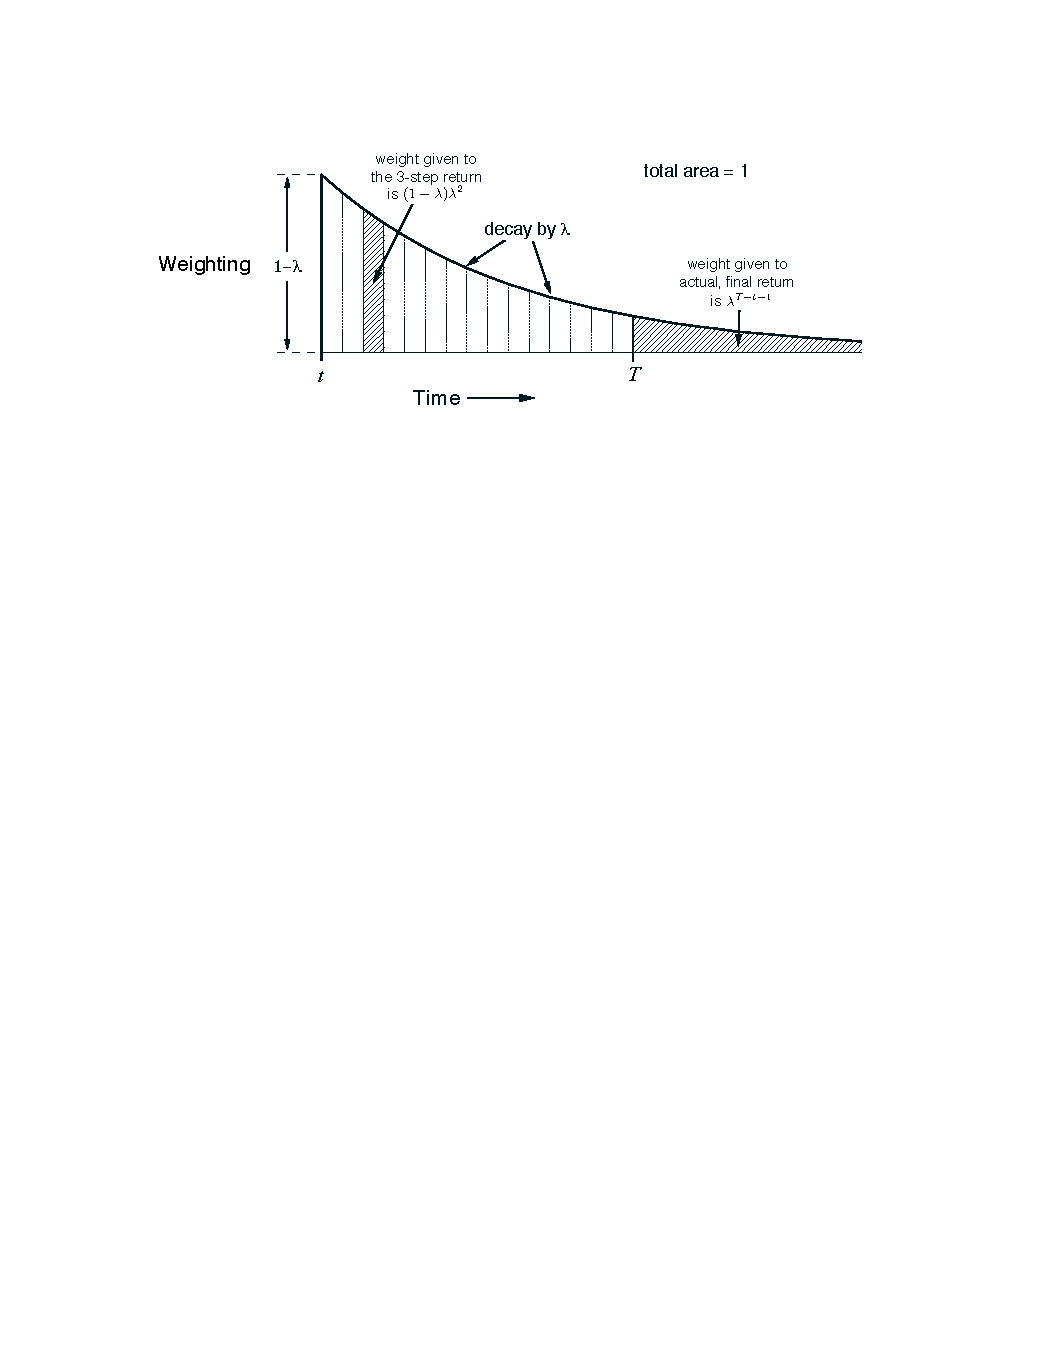
\includegraphics[height=0.275\textheight]{fig/lec06/Lambda_Weighting_Series.pdf}
\caption{Weighting overview in $\lambda$-return series (source: R. Sutton and G. Barto, Reinforcement learning: an introduction, 2018, \href{https://creativecommons.org/licenses/by-nc-nd/2.0/}{CC BY-NC-ND 2.0})}
\label{fig:Lambda_Weighting_Series}
\end{figure}}
}

%%%%%%%%%%%%%%%%%%%%%%%%%%%%%%%%%%%%%%%%%%%%%%%%%%%%%%%%%%%%%
%% Truncated $\lambda$-Returns %%
%%%%%%%%%%%%%%%%%%%%%%%%%%%%%%%%%%%%%%%%%%%%%%%%%%%%%%%%%%%%%
\frame{\frametitle{Truncated $\lambda$-returns for continuing tasks}
\begin{itemize}
	\item Using $\lambda$-returns as in \eqref{eq:lambda_return} is not feasible for \hl{continuing tasks}.
	\item One would have to wait infinitely long to receive the trajectory.\pause
	\item Intuitive approximation: \hl{truncate $\lambda$-return after $h$ steps} 
	\begin{equation}
		g_{k:h}^\lambda = (1-\lambda)\sum_{n=1}^{h-k-1}\lambda^{(n-1)}g_{k:k+n} + \lambda^{h-k-1}g_{k:h}\,.
		\label{eq:lambda_return_trunc}
	\end{equation}
	\item Horizon $h$ divides continuing tasks in rolling episodes.
\end{itemize}
}

%%%%%%%%%%%%%%%%%%%%%%%%%%%%%%%%%%%%%%%%%%%%%%%%%%%%%%%%%%%%%
%% Forward View %%
%%%%%%%%%%%%%%%%%%%%%%%%%%%%%%%%%%%%%%%%%%%%%%%%%%%%%%%%%%%%%
\frame{\frametitle{Forward view}
\onslide<1->{\begin{itemize}
	\item Both, $n$-step and $\lambda$-return updates, are based on a forward view.  
	\item We have to wait for future states and rewards to arrive before we are able to perform an update.}
	\onslide<2->{\item Currently, $\lambda$-returns are only an alternative to $n$-step updates with different weighting options.}
\end{itemize}
\onslide<1->{\begin{figure}
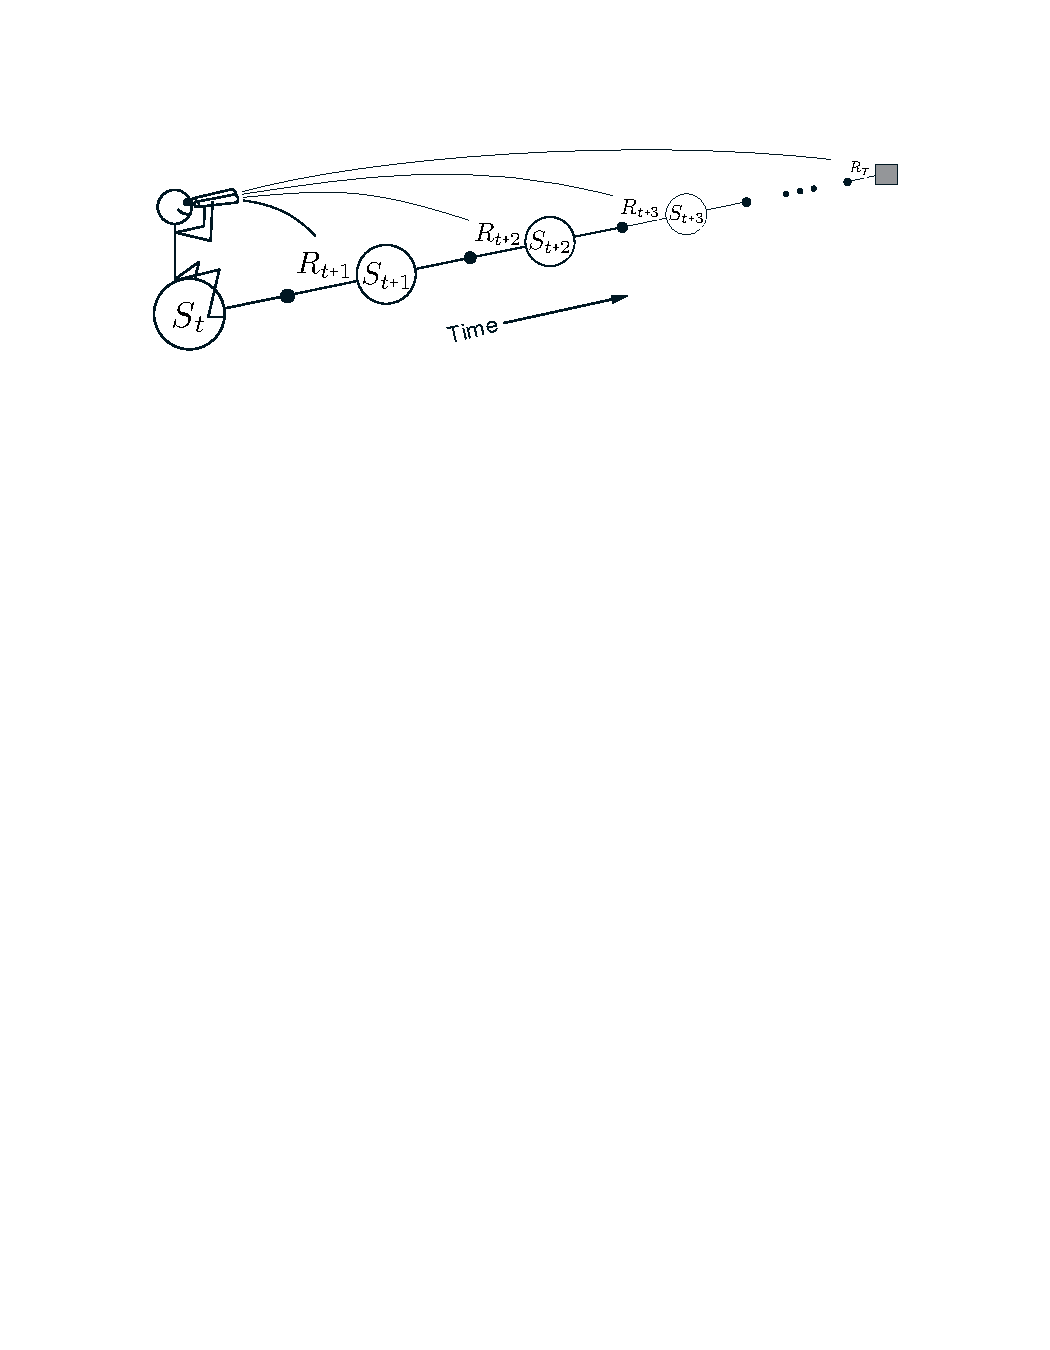
\includegraphics[height=0.25\textheight]{fig/lec06/Forward_View.pdf}
\caption{The forward view: an update of the current state value is evaluated by future transitions (source: R. Sutton and G. Barto, Reinforcement learning: an introduction, 2018, \href{https://creativecommons.org/licenses/by-nc-nd/2.0/}{CC BY-NC-ND 2.0})}
\label{fig:Forward_View}
\end{figure}}
}

%%%%%%%%%%%%%%%%%%%%%%%%%%%%%%%%%%%%%%%%%%%%%%%%%%%%%%%%%%%%%
%% Backward View %%
%%%%%%%%%%%%%%%%%%%%%%%%%%%%%%%%%%%%%%%%%%%%%%%%%%%%%%%%%%%%%
\frame{\frametitle{Backward view of TD($\lambda$)}
\onslide<1->{General idea:
\begin{itemize}
	\item Use $\lambda$-weighted returns looking into the past. 
	\item Implement this in a recursive fashion to save memory.}
	\onslide<2->{\item Therefore, an \hl{eligibility trace $z_k$} denoting the importance of past events to the current state update is introduced. }
\end{itemize}
\onslide<1->{\begin{figure}
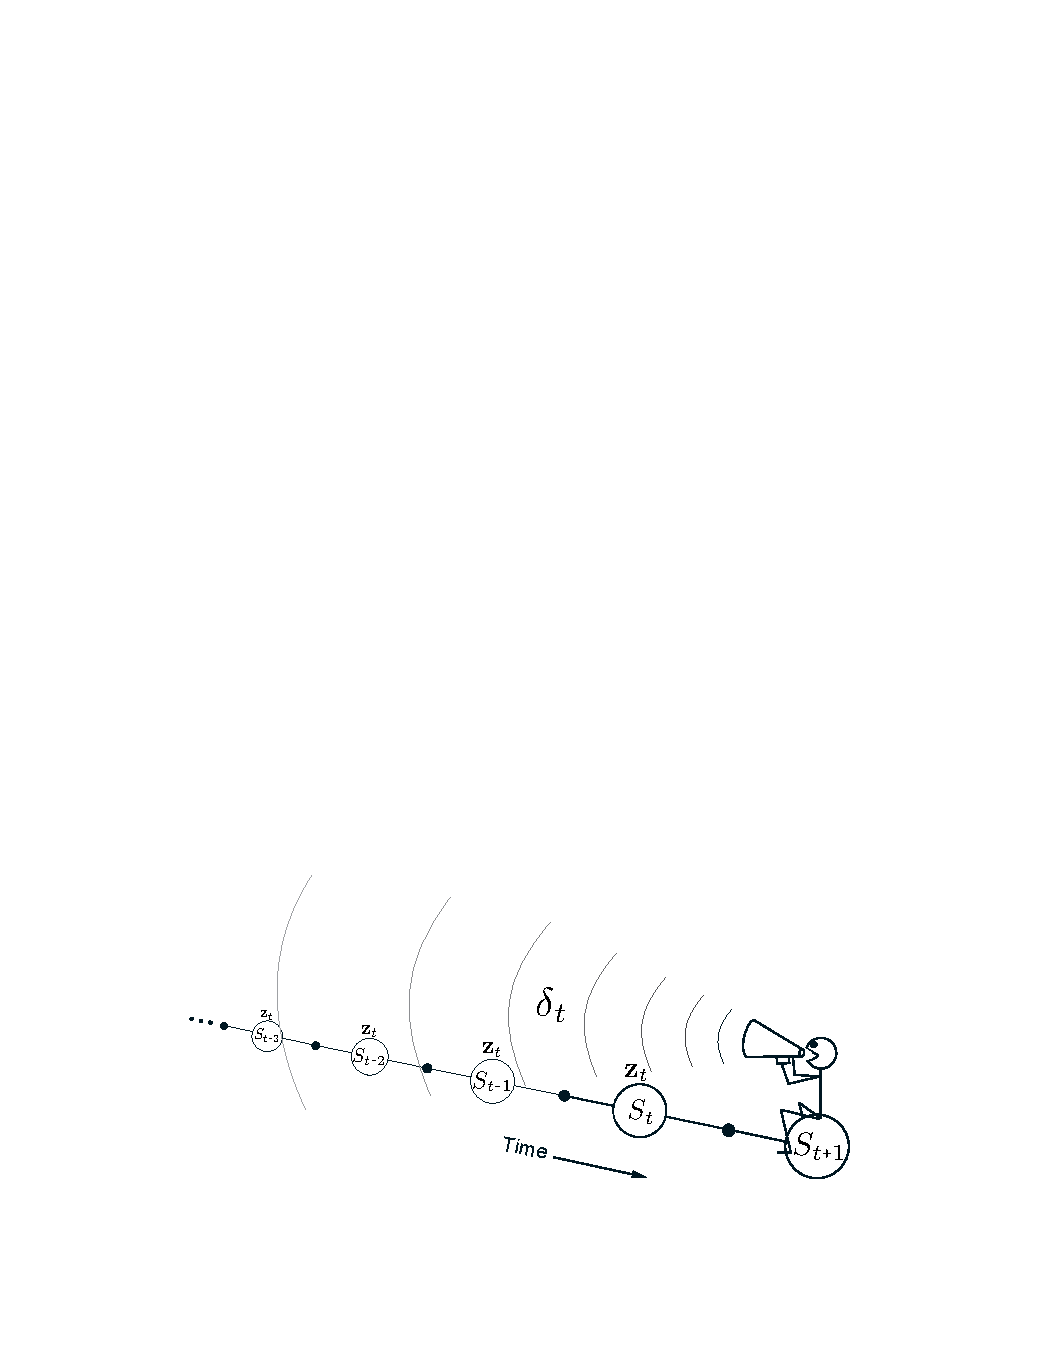
\includegraphics[height=0.4\textheight]{fig/lec06/Backward_View.pdf}
\caption{The backward view: an update of the current state value is evaluated based on a trace of past transitions (source: R. Sutton and G. Barto, Reinforcement learning: an introduction, 2018, \href{https://creativecommons.org/licenses/by-nc-nd/2.0/}{CC BY-NC-ND 2.0})}
\label{fig:Backward_View}
\end{figure}}
}

%%%%%%%%%%%%%%%%%%%%%%%%%%%%%%%%%%%%%%%%%%%%%%%%%%%%%%%%%%%%%
%% Eligibility Trace (1) %%
%%%%%%%%%%%%%%%%%%%%%%%%%%%%%%%%%%%%%%%%%%%%%%%%%%%%%%%%%%%%%
\frame{\frametitle{Eligibility trace (1)}
Why is the exponential weighting particular suitable for TD($\lambda$)?\pause
\begin{itemize}
	\item Because we can easily implement this in a recursive fashion.\pause
\end{itemize}
\begin{block}{Exponential smoothing filter}
Let $x_k$ be an arbitrary signal sampled at equally distributed time steps $k$. Then, the filtered signal $y_k$ with an exponential window function of past observations is
\begin{equation}
	y_k = \beta x_k + (1-\beta)y_{k-1}, \quad k> 0 \quad \mbox{and} \quad y_0=x_0
	\label{eq:exp_smoothing_filter}
\end{equation}
with $\beta\in\{\mathbb{R}|0<\beta<1\}$ being the smoothing factor.  
\end{block}\pause
\begin{itemize}
	\item Above is a simple recursive exponential smoothing filter which converges for $k>>1$.
\end{itemize}
}

%%%%%%%%%%%%%%%%%%%%%%%%%%%%%%%%%%%%%%%%%%%%%%%%%%%%%%%%%%%%%
%% Eligibility Trace (2) %%
%%%%%%%%%%%%%%%%%%%%%%%%%%%%%%%%%%%%%%%%%%%%%%%%%%%%%%%%%%%%%
\frame{\frametitle{Eligibility trace (2)}
The \hl{eligibility trace $z_k(x)\in\mathbb{R}$} is defined and tracked for each state $x$ separately:
	\begin{equation}
\begin{split}
	z_{0}(x)&=0,\\
	z_k(x) &=\gamma\lambda z_{k-1}(x)+\begin{cases}0, \quad\mbox{if } x_k \neq x, \\ 1, \quad \mbox{if } x_k = x.\end{cases}
\end{split}	
\label{eq:Elig_trace}
\end{equation}
\begin{figure}
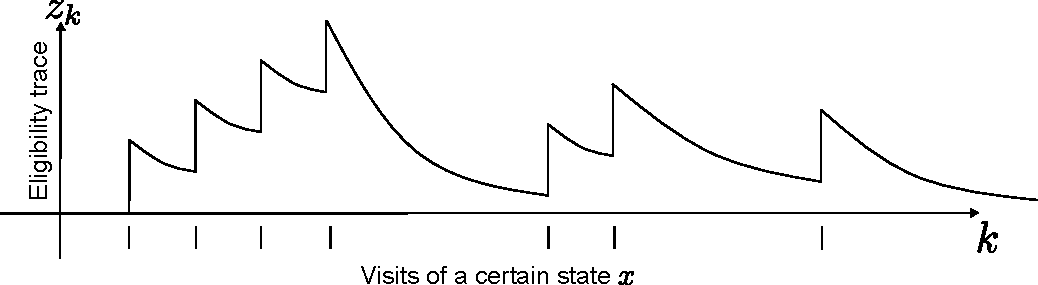
\includegraphics[height=0.36\textheight]{fig/lec06/State_Visits_Eligibility_Trace.pdf}
\caption{Simplified representation of updating an eligibility trace of an arbitrary state in a finite MDP}
\label{fig:State_Visits_Eligibility_Trace}
\end{figure}
}

%%%%%%%%%%%%%%%%%%%%%%%%%%%%%%%%%%%%%%%%%%%%%%%%%%%%%%%%%%%%%
%% TD($\lambda$) updates using eligibility traces %%
%%%%%%%%%%%%%%%%%%%%%%%%%%%%%%%%%%%%%%%%%%%%%%%%%%%%%%%%%%%%%
\frame{\frametitle{TD($\lambda$) updates using eligibility traces}
Based on the eligibility trace definition from \eqref{eq:Elig_trace} we can modify our value estimates:
\begin{block}{TD($\lambda$) state-value update}
The TD($\lambda$) state-value update is:
\begin{equation}
		\hat{v}(x_k) \leftarrow \hat{v}(x_k) + \alpha \left[r_{k+1} + \gamma \hat{v}(x_{k+1})- \hat{v}(x_k)\right]z_k(x_k).
\end{equation}
\end{block}

\begin{block}{TD($\lambda$) action-value update}
	The TD($\lambda$) action-value update is:
		\begin{equation}
		\hat{q}(x_k, u_k) \leftarrow \hat{q}(x_k, u_k) + \alpha\left[r_{k+1}+\gamma\hat{q}(x_{k+1}, u_{k+1}) - \hat{q}(x_k, u_k)\right]z_k(x_k) .
		\end{equation}
\end{block}
Already known prediction and control methods can be modified accordingly. In contrast to $n$-step forward updates, one can conclude:
\begin{itemize}
	\item Advantage: recursive updates based on past updates (no additional waiting time),
	\item Disadvantage: effort for storing an eligibility trace for each state (scaling problem).
\end{itemize}
}

%%%%%%%%%%%%%%%%%%%%%%%%%%%%%%%%%%%%%%%%%%%%%%%%%%%%%%%%%%%%%
%% Sarsa Learning Comparison in Gridworld Example %%
%%%%%%%%%%%%%%%%%%%%%%%%%%%%%%%%%%%%%%%%%%%%%%%%%%%%%%%%%%%%%
\frame{\frametitle{SARSA learning comparison in gridworld example}
\begin{itemize}
	\item $\lambda$ can be interpreted as the discounting factor acting on the eligibility trace (see right-most panel below).
	\item Intuitive interpretation: more recent transitions are more certain/relevant for the current update step. 
\end{itemize}
\vspace{0.3cm}
\begin{figure}
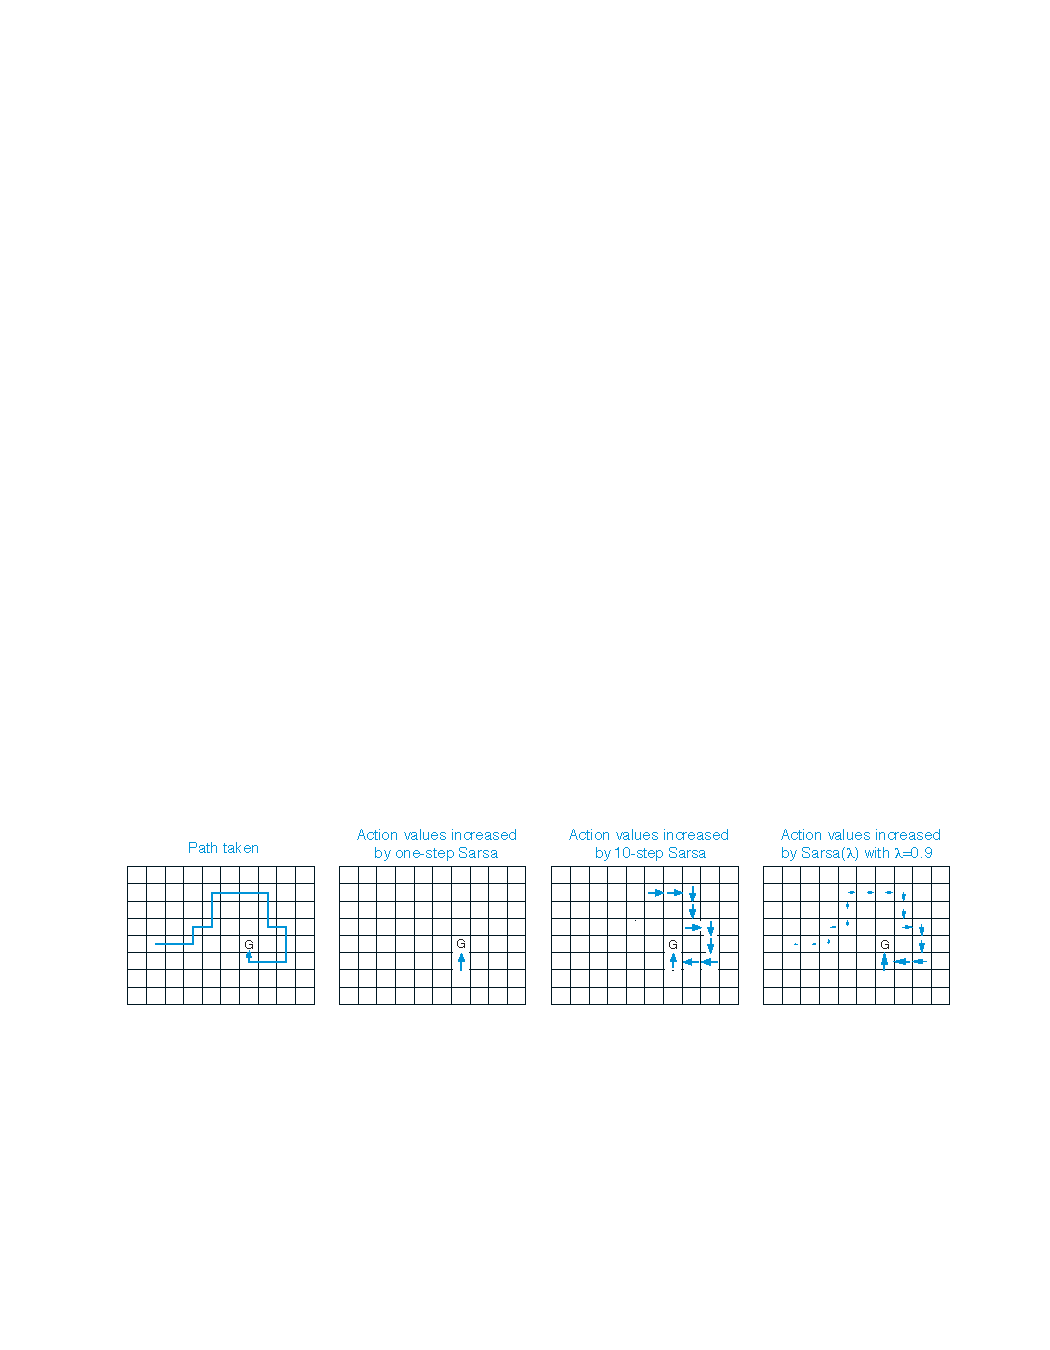
\includegraphics[height=0.4\textheight]{fig/lec06/Traces_Sarsa_Gridworld.pdf}
\caption{SARSA variants after an arbitrary episode within a gridworld environment -- arrows indicate action-value change starting from initially zero estimates (source: R. Sutton and G. Barto, Reinforcement learning: an introduction, 2018, \href{https://creativecommons.org/licenses/by-nc-nd/2.0/}{CC BY-NC-ND 2.0})}
\label{fig:Traces_Sarsa_Gridworld}
\end{figure}
}


%%%%%%%%%%%%%%%%%%%%%%%%%%%%%%%%%%%%%%%%%%%%%%%%%%%%%%%%%%%%%
%% Summary %%
%%%%%%%%%%%%%%%%%%%%%%%%%%%%%%%%%%%%%%%%%%%%%%%%%%%%%%%%%%%%%
\begin{frame}
\frametitle{Summary: what you've learned today}
\begin{itemize}
	\item $n$-step updates allow for an intermediate solution in between temporal difference and Monte Carlo:
	\begin{itemize}
		\item $n=1$: TD as special case,
		\item $n=T$: MC as special case.
	\end{itemize}\pause
	\item The parameter $n$ is a delicate degree of freedom:
	\begin{itemize}
		\item It contains a trade-off between the learning delay and uncertainty reduction when considering more or less steps.
		\item Choosing it is non-trivial and sometimes more art than science.
	\end{itemize}
	\item $\lambda$-returns lead to compound updates which introduce an exponential weighting to visited states.
	\begin{itemize}
		\item Rationale: states which have been already visited long ago are less important for the current learning step.
	\end{itemize}
	\item TD($\lambda$) transfers this idea into a recursive, backward oriented approach.
	\begin{itemize}
		\item Eligibility traces store the long-term visiting history of each state in a recursive fashion.
	\end{itemize}
\end{itemize}
\end{frame}